\documentclass[12pt,letterpaper, onecolumn]{exam}
\usepackage{amsmath}
\usepackage{amssymb}
\usepackage{algorithm}
\usepackage{algorithmic}
\usepackage[]{algorithm2e}
\usepackage{graphicx}
\usepackage[lmargin=71pt, tmargin=1.2in]{geometry}  %For centering solution box

% \chead{\hline} % Un-comment to draw line below header
\thispagestyle{empty}   %For removing header/footer from page 1

\begin{document}

\begingroup  
    \centering
    \LARGE COT5405 Analysis of Algorithms\\
    \LARGE Assignment 1\\[0.5em]
    \large \today\\[0.5em]
    \large Sankalp Pandey\par
    \large UFID: 92878142\par
\endgroup
\rule{\textwidth}{0.4pt}
\pointsdroppedatright   %Self-explanatory
\printanswers
\renewcommand{\solutiontitle}{\noindent\textbf{Ans:}\enspace}   %Replace "Ans:" with starting keyword in solution box
\begingroup
    \centering
    \LARGE \textbf{Section 1}\\
\endgroup
\vspace{16pt}
\par[50 marks] As part of this problem, you have to design and implement an algorithm to find a cycle (just one cycle) in an undirected graph.
\begin{questions}

    \question Design a correct algorithm and show it in pseudo-code [10]\droppoints
    
    \begin{solution}
    \\
        ( bool array visited of size number of vertex in graph with all values false )\\
        ( stack cycle to fill all vertex of cycle deteted )\\
        
        \begin{algorithm}[H]
        \SetKwFunction{FMain}{FindCycle}
        \SetKwProg{Fn}{Function}{:}{}
        \Fn{\FMain{$source$,$parent$,$visited$,$cycle$,$graph$}}{
           $ visited[source] \leftarrow true$\\
            push cycle, source\\
            \For{each vertex $v\in graph[source]$}{
                \uIf{visited[v] == false}{
                    \uIf{FindCycle(v, source, visited, cycle, graph) == true}{
                        \Return true
                    }
                    \uElseIf{$parent \neq v$}{
                        push cycle, v\\
                        \Return true
                    }
                } 
            }
            pop cycle\\
            \Return false\\
        }
        \textbf{End Function}
        \caption{Algorithm to find cycle in an undirected graph}
        \label{FindCycleAlgo} 
        \end{algorithm}
    \end{solution}
    \pagebreak %Not necessary
    \question Provide proof of the algorithm's correctness [10]
    
    \begin{solution}
        \\
        \begin{parts}
        
        \part Proof by contradiction:\\
        Suppose that the above graph G(V,E) does not contain cycle and $u\in adj(v)$ and $v\in adj(u)$ and $v-1 \in adj(u)$\\
        We start at a source vertex u and keep a boolean array to mark already visited vertices. We also maintain a parent pointer to keep track of parent of any vertex at any point of time. Now when we reach at vertex v, the parent contains v-1 if v is not visited. If v is not visited then no visited vertices before v-1 can have an edge with it. But we know that $u\in adj(v)$ from our representation. This means that graph G(V,E) has a cycle.\\
        \\
        Proof of termination:\\
        \\
        Case 1: If cycle exists\\
        DFS algorithm will traverse each vertex once and push it to stack. If vertex is visited and the parent of previous vertex is not equal to current vertex, algorithm terminates with stack containing cycle nodes.\\
        
        Case 2: If cycle doesn't exists\\
        DFS algorithm traverse each vertex once and pushes the vertex in stack. If it doesn't finds cycle, it will pop each element and algorithm terminates with empty stack.
         
    
    
        
            
    \end{parts}
    \end{solution}
            \begin{figure}
            \centering
            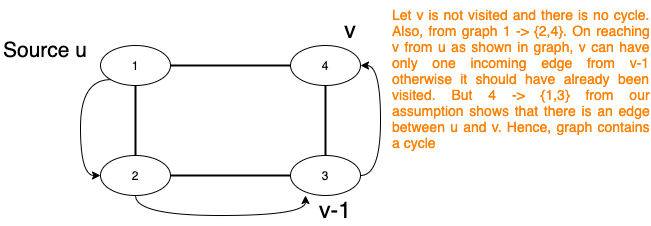
\includegraphics[width=14cm]{cycle_proof.drawio.png}
            \caption{Proof of cycle detection visualization}
            \label{fig:galaxy}
            \end{figure}
    \pagebreak %Not necessary
    
    \question Find and prove the algorithm's running time [10]\droppoints
    
    \begin{solution}
    \\
            \textbf{$|V|$ is number of vertex and $|E|$ is number of edges}
            \begin{algorithm}[H]
            \SetKwFunction{FMain}{FindCycle}
            \SetKwProg{Fn}{Function}{:}{}
            \Fn{\FMain{$source$,$parent$,$visited$,$cycle$,$graph$}}{
                $ visited[source] \leftarrow true$  \hspace{225pt}     \textbf{O(1)}\\
                push cycle, source   \hspace{250pt} \textbf{O(1)}\\
                
                \For{each vertex $v\in graph[source]\hspace{145pt}     \textbf{O($|V|+|E|$)}$}{  
                    \uIf{visited[v] == false}{
                        \uIf{FindCycle(v, source, visited, cycle, graph) == true}{
                            \Return true
                        }
                        \uElseIf{$parent \neq v$}{
                            push cycle, v\\
                            \Return true
                        }
                    } 
                } 
                pop cycle \hspace{295pt} \textbf{O(1)}\\
                \Return false\\
            }
            \textbf{End Function}
            \label{FindCycleAlgo} 
            \end{algorithm}
            The running time of above algorithm is \textbf{O($|V|+|E|$)}. This is because in the above adjacency list representation of graph we discover each vertex and its neighbours exactly once. The time complexity to discover a vertex is O(1) and for its neighbours is O(degree(vertex)). In worst case, we discover all vertices to find a cycle. Hence, the time complexity will be:\\
            $\Sigma(1+degree(i))$ where $1<=i<=V$\\
            $\Sigma(degree(i)) = 2E$ as in an undirected graph there is incoming and outgoing edge from a vertex\\
            Hence, time complexity will be O($|V|+2|E|$) $\sim$ O($|V|+|E|$)
    \end{solution}
    \pagebreak %Not necessary
    \question Implement the algorithm in a compiled language and: [20]\droppoints
        \begin{solution}
            \begin{parts}
                    \part Write a graph generator (Hint: use an existing graph generation library if you can)\\
                    Code attached in zip file
                    \part Write test code to validate that the algorithm finds cycles\\
                    Code attached in zip file
                    \part Test the algorithm for increasing graph sizes.\\
                    Code attached in zip file
                    \part Plot the running time as a function of size to verify that the asymptotic complexity in step 3 matches experiments\\
                    \\
                    \textbf{How to run above the code in zip file}\\
                    1. In terminal go to folder location where file $one\_cycle.cpp$ is present.\\
                    2. Run $\textbf{make one\_cycle}$. This will generate executable file $\textbf{one\_cycle}$.\\
                    3. Run $\textbf{./one\_cycle}$ to run the code.\\
                    4. Commandline will ask user to enter 1 for running algorithm and enter 2 to run the test code. Enter 1.\\
                    5. Next, commandline will ask to enter number of vertices. Enter 100.\\
                    6. Now commandline will ask to enter number of edges. Enter 200.\\
                    7. Algorithm will run to find a cycle. If cycle found, it will display the vertices of the cycle.\\
                    8. Run $\textbf{./one\_cycle}$ again. This time enter 2 to run testcode. Two test cases will run to show when cycle is present and other when cycle is not present.
                    
            \end{parts}
        \end{solution}
        
        \end{questions}
        \begin{figure}
            \centering
            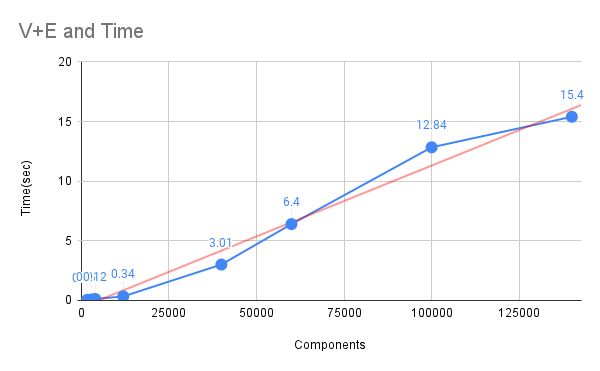
\includegraphics[width=14cm]{chart1.png}
            \caption{Plot of running time as a function of size}
            \label{fig:galaxy}
        \end{figure}
    \pagebreak %Not necessary
    
    \begingroup
        \centering
        \LARGE \textbf{Section 2}\\
    \endgroup
\vspace{16pt}
\par For this problem, we consider undirected graphs that have n nodes and at most n+8 edges. For these graphs, you have to design an efficient algorithm that finds the minimum spanning tree.
\begin{questions}
\question Design a correct algorithm and show it in pseudo-code [10]\droppoints
\begin{solution}
    \begin{algorithm}[H]
        \SetKwFunction{FMain}{FindMinimumSpanningTree}
        \SetKwProg{Fn}{Function}{:}{}
        \Fn{\FMain{$Edges[]$ E, $vCount$}}{
            \Return if graph E is not connected\\
            sort graph E based on decreasing order of edge weight\\
            \For{$i\leftarrow 0$ ; $i<size(E)$ ; $i\leftarrow i+1$}{
                $edge \leftarrow E[i]$\\
                \textbf{delete} edge \\
                \uIf{graph is not connected}{
                    $E[i]\leftarrow edge$
                }
            }
            \Return E
        }
        \vspace{12pt}
        \textbf{End Function}
        \caption{Algorithm to find minimum spanning tree}
        \label{MinimumSpanningTreeAlgo} 
        \end{algorithm}
\end{solution}
        \begin{figure}
            \centering
            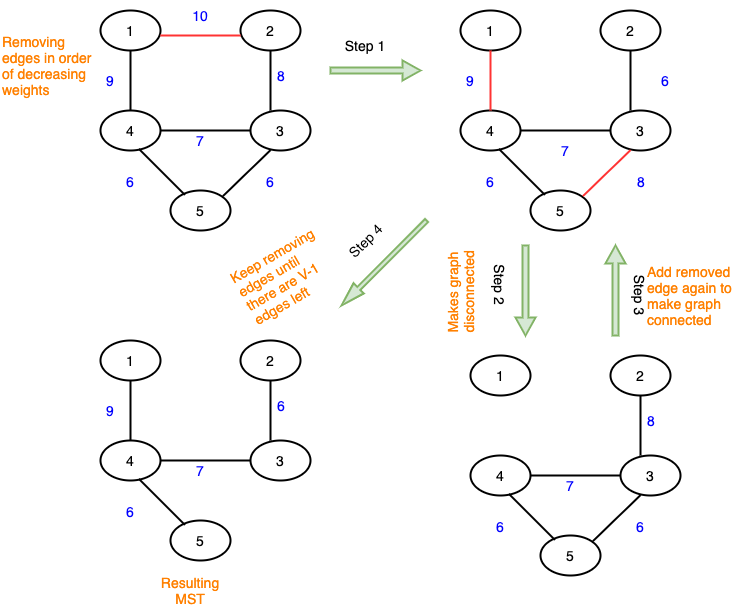
\includegraphics[width=14cm]{mstalgo.png}
            \caption{Algorithm to find minimum spanning tree}
            \label{fig:galaxy}
        \end{figure}
\pagebreak
\question Provide proof of the algorithm's correctness [10]
\begin{solution}
\\
The provided algorithm deletes edges in order of
decreasing cost. When any edge is removed the graph stays
connected so it has be the most expensive edge on a cycle.
The edges which are removed do not belong to any minimum spanning tree. The  algorithm removes all cycles by deleting the most expensive edges. All edges that do not belong to a minimum spanning tree are removed.\\
When any edge is removed which causes the graph to become disconnected, it is replaced back in the graph. The  algorithm does not remove any edges that causes graph to become disconnected. The graph produced by the algorithm has no cycles and is connected. The resulting graph is a tree and a minimum spanning tree.\\
\\
Proof of correctness:\\
Part1: Resulting graph after edges deletion is a spanning tree
The resulting sub-graph from the algorithm is not disconnected as we are checking that in our algorithm. There is no cycle present since if it does then while iterating over the edges we would encounter the max edge in the cycle and we would delete that edge. Thus, resulting graph is a minimum spanning tree of original graph.\\
\\
Part2: Minimality - Proof by induction:\\
If F is a set of edges remained after delete operations then there must be a spanning tree $T \subset F$. This is true as F contains all the edges and each weighted graph has a minimum spanning tree and thus it will be subset of F.\\
Let F be a non-final set of edges and $T\subset F$ be a minimum spanning tree, we need to show that after deleting an edge e in our algorithm, there exists a minimum spanning tree $T' \subset F$\\
1. If next deleted edge $e \notin T$ then $T=T' \subset F$. Hence, proved.\\
2. If $e \in T$. Deleting e causes T to become disconnected. Assume e separates T into sub-graphs S and V. Since the whole graph is connected after deleting e then there must exists a path between S and V so there must exist a cycle C in the F (before removing e). now we must have another edge in this cycle $f \notin T$ but $f \in F$ (since if all the cycle edges were in tree T then it would not be a tree anymore). So we show that T' = T - e + f is the minimum spanning tree $\subset$ F. 
\end{solution}
\pagebreak
\question Find and prove the algorithm's running time [10]
\begin{solution}
\begin{algorithm}[H]
        \SetKwFunction{FMain}{FindMinimumSpanningTree}
        \SetKwProg{Fn}{Function}{:}{}
        \Fn{\FMain{$Edges[]$ E, $vCount$}}{
            \Return if graph is not connected\\
            sort graph E based on decreasing order of edge weight \hspace{50pt}\textbf{O($|E|log(|E|)$}\\
            \For{$i\leftarrow 0$ ; $i<size(E)$ ; $i\leftarrow i+1$}{
                $edge \leftarrow E[i]$\hspace{240pt}\textbf{O($|E|$)}\\
                \textbf{delete} edge \hspace{235pt}\textbf{O(1)}
                
                \uIf{graph is not connected \hspace{160pt}\textbf{O($|V|+|E|$)}}{
                    $E[i]\leftarrow edge$ \hspace{220pt}\textbf{O(1)}
                }
            }
            \Return E
        }
        \vspace{12pt}
        \textbf{End Function}
        \label{MinimumSpanningTreeAlgo} 
        \end{algorithm}
        The running time of above algorithm is:\\ \textbf{O($|E|log|E|$)+O(1)+O($|E|$)*(O(1)+O($|V|+|E|$)+O(1)) $\sim$ O($|E|\wedge 2$)}\\
        The time complexity of this algorithm can be made more efficient by 
        improving the complexity of algorithm to find graph connectivity to \textbf{O($mlogn(log logn \wedge 3$))} as given by Mikkel Thorup
\end{solution}
\pagebreak
\question Implement the algorithm in a compiled language and: [20]
\begin{solution}
    \begin{parts}
                    \part Write a graph generator (Hint: use an existing graph generation library if you can)\\
                    Code attached in zip file
                    \part Write test code to validate that the algorithm finds cycles\\
                    Code attached in zip file
                    \part Test the algorithm for increasing graph sizes.\\
                    Code attached in zip file
                    \part Plot the running time as a function of size to verify that the asymptotic complexity in step 3 matches experiments \\
                    \\
                    \textbf{How to run above the code in zip file}\\
                    1. In terminal go to folder location where file $mst.cpp$ is present.\\
                    2. Run $\textbf{make mst}$. This will generate executable file $\textbf{mst}$.\\
                    3. Run $\textbf{./mst}$ to run the code.\\
                    4. Commandline will ask user to enter 1 for running algorithm and enter 2 to run the test code. Enter 1.\\
                    5. Next, commandline will ask to enter number of vertices. Enter 5.\\
                    6. Now commandline will ask to enter number of edges. Enter 13.\\
                    7. Algorithm will run to find a mst and minimum cost. The algorithm will return minimum cost or -1 if graph is not connected.\\
                    8. Run $\textbf{./mst}$ again. This time enter 2 to run testcode. Testcase will show that minimum cost is same as actual result.
                    
            \end{parts}
\end{solution}

\end{questions}
\begin{figure}
            \centering
            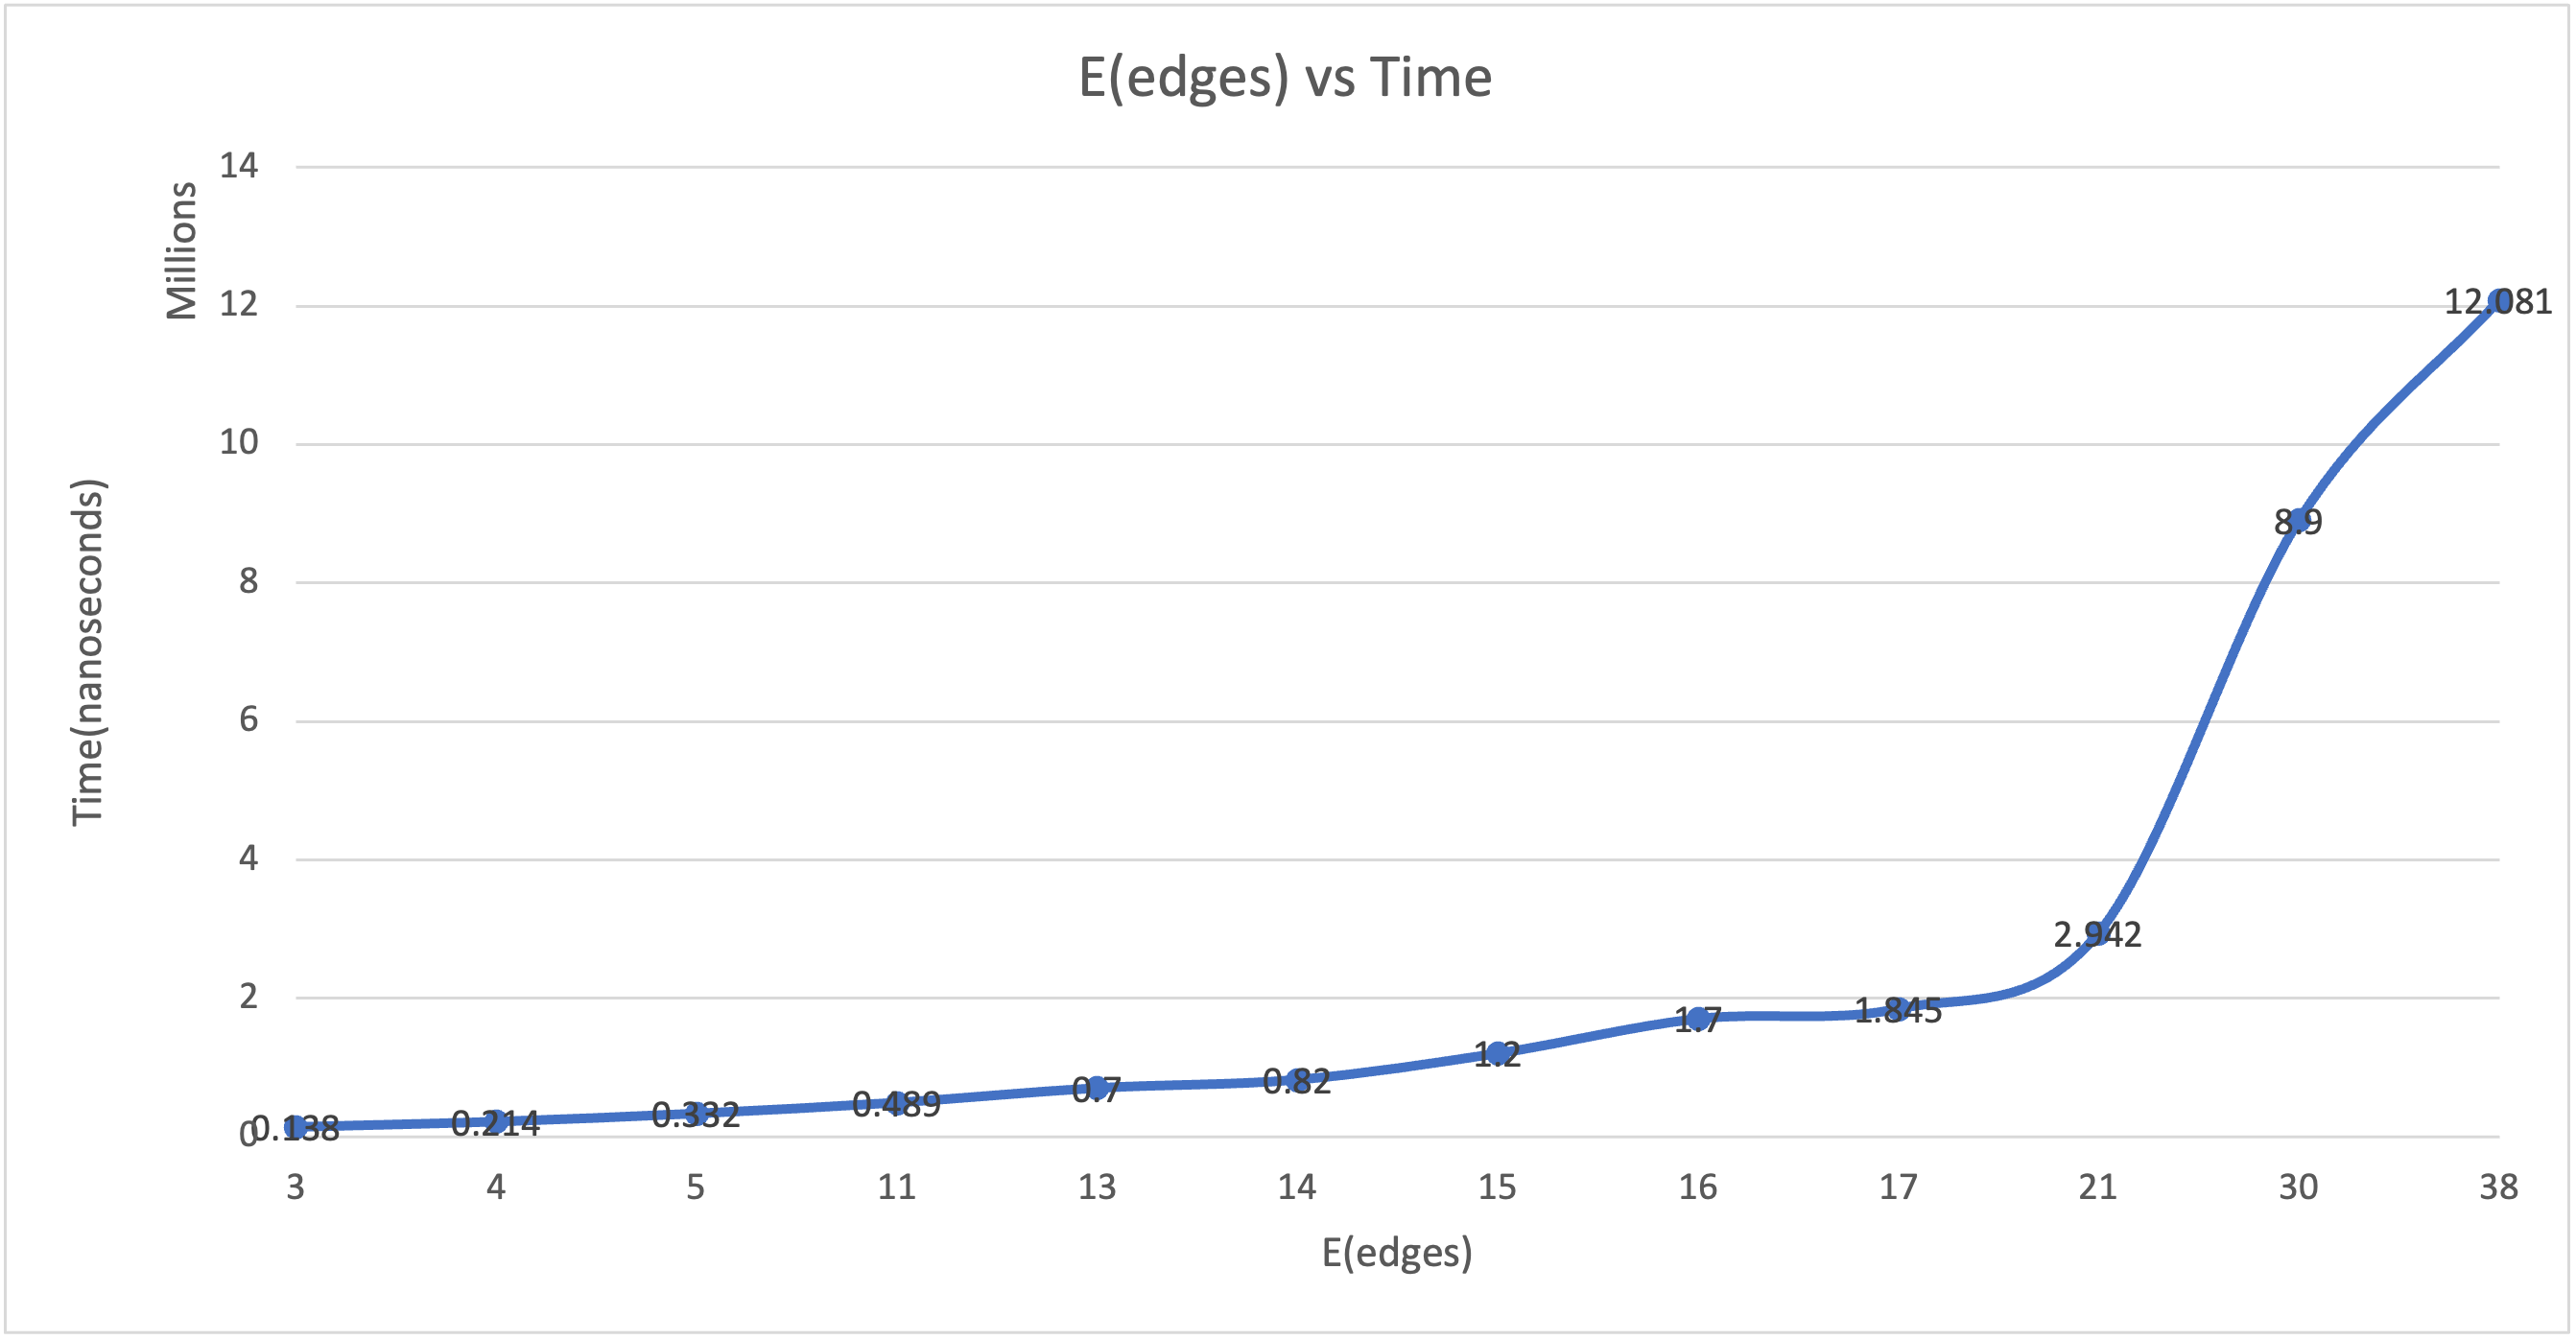
\includegraphics[width=14cm]{Picture1.png}
            \caption{Plot of MST running time as a function of E(edges)}
            \label{fig:galaxy}
        \end{figure}


\end{document}